\chapter{Music}
\section{Major scale}
There are three way to generate the major scale
\begin{itemize}
	\item Pythagorean scale
	\item Just scale
	\item Temperate scale
\end{itemize}

\subsection{Pythagorean scale}
Builds the major scale using the first and second harmonic; respectively double and triple of base note or octave and fifth (one octave too high).

The notes are obtained in this order: C - G - D - A - E - B. F is found by going downward. 

\subsubsection{Pythagorean comma}
With this method we found an inconsistency (called pythagorean comma).

If we go up 7 octaves or 12 fifth, we should theoretically find the same frequency, but we don't. 
\begin{equation}
	\frac{\frac{2}{3}^{12}}{2^7}=\frac{3^{12}}{2^{19}}\neq 1
\end{equation}

\subsection{Just Scale}
Uses octave (2nd harmonic), fifth (third harmonic) and third (fifth harmonic).

There is an inconsistency between this method and the pythagorean. Here a third is $\frac{5}{4}$ whereas in the case of the pythagorean scale it is $\frac{81}{64}$.




\section{Note Generator}
A note can be generated as following

\begin{eqnarray}
	f[n+k]=f[n]\cdot2^{\frac{k}{12}}
\end{eqnarray}
where $f[n]$ is the frequency of a note and $k$ is the number of half-tone above this note.

For instance, if one wants to calculate the frequency of a C, beginning with the frequency of an A (440 hz), he must add three half tones to A thus with $f[0]=440 Hz$ we have

\begin{eqnarray*}
	f_C=f_A[3]=440\cdot2^{3/12}=440\cdot2^{1/4}\approx 523.25 Hz
\end{eqnarray*}

\begin{table}
	\begin{tabular}{c | c}
		Note & Freq [Hz] \\
		\hline
		A & 440.0000 \\		
		Bb &  466.1638\\
		B &  493.8833\\
		C & 523.2511\\
		Cs &  554.3653\\
		D &   587.3295\\
		Eb &  622.2540\\
		E &  659.2551\\
		F &  698.4565\\
		Fs &  739.9888\\
		G &  783.9909\\  
		Ab & 830.6094\\
	  	A & 880.0000 \\
	\end{tabular}
	\caption{One octave of notes with their respective frequencies. Note that the octave is exactly twice the fundamental's frequency}
\end{table}


\begin{table}
	\begin{tabular}{l|c | c | c}
		&Pythagorean  & Just & Temperate \\
		\hline
		C & 1 & 1 & 1 \\		
		D &  $9/8$ & $9/8$ &$2^{\frac{2}{12}}$\\
		E & $81/64$ & $5/4$ & $2^{\frac{4}{12}}$\\
		F & $4/3$ & $4/3$ & $2^{\frac{5}{12}}$\\
		G & $3/2$ &$3/2$ & $2^{\frac{7}{12}}$\\
		A &   $27/16$ &$5/3$ & $2^{\frac{9}{12}}$\\
		B &  $243/128$ & $15/8$ & $2^{\frac{11}{12}}$\\
		C &  $2$ & $2$ & $2^{\frac{12}{12}}=2$\\
	\end{tabular}
	\caption{One octave of notes with their respective frequencies. Note that the octave is exactly twice the fundamental's frequency}
\end{table}

\begin{figure}[h!]
  \centering
    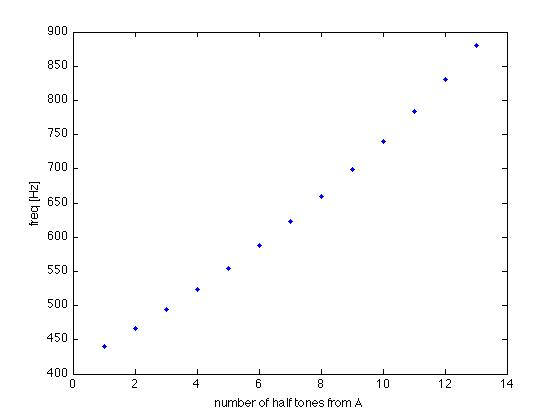
\includegraphics[width=0.8\textwidth]{images/music_freq_distribution.jpg}
  \caption{Distribution of the notes with respect to their frequency}
\end{figure}
